\documentclass{beamer}
\usetheme{metropolis} % Use metropolis theme
\usepackage[utf8]{inputenc}
\usepackage[portuguese]{babel}
\usepackage{lipsum}
\usepackage{ragged2e}
\usepackage{etoolbox}
\usepackage{graphicx}


\title{Simulador de processos}
\date{\today}
\author{Luis e Gabriel}
\institute{Centre for Modern Beamer Themes}
\begin{document}
\maketitle

\section{Considerações Escalonador}
\begin{frame}{Princípios}
	\begin{itemize}
		\item Um processo somente pode ser criado a partir de outro.
		\item A o escalonador deve ter um processo em sua fila antes de iniciar.
		\item Se não há nenhum processo a ser executado, desligamos todos as CPUs.
	\end{itemize}
\end{frame}


\begin{frame}{Como Implementamos}
	Os três tipos de escalonadores devem apresentar as seguintes funções:
	\begin{itemize}
		\item \textsc{p\_init}: função chamada para ligar o nosso escalonador. Ela verifica quantas CPUs há no computador do usuário e inicia uma thread para cada uma. Finaliza somente quando não há mais processos a serem executados.
		\item \textsc{p\_exec}: recebe as características de um novos processo (nome, linha do trace, tempo de execução, ponteiro para função e argumentos da função). Adiciona esse processo ao escalonador.
		\item \textsc{p\_run}: chamada dentro de um processo, verifica se ele deve continuar sua execução ou parar.
	\end{itemize}
\end{frame}


\begin{frame}{Processo \textsc{load\_process} (-1)}
	\justifying
	Antes do nosso escalonador iniciar, adicionamos esse processo a ele. Esse processo tem a função criar os nossos outros processos. Ou seja, ele verifica se já está na hora de adicionar outros processos no escalonador baseado no arquivo de trace. 
	
	Quando existe processo pedentes a serem criados, ele espera 0,5s e depois adiciona a sí mesmo no escalonador. 
\end{frame}


\begin{frame}{Exemplo}
	Vamos executar esse exemplo com os 4 algorítimos e pintar cada processo com uma cor.
	\begin{columns}[T,onlytextwidth]
		\column{0.5\textwidth}
		
		0 1 processo1 20 \newline
		0 2 processo2 20 \newline
		0 3 processo3 20 \newline
		0 4 processo4 20 \newline
		1 5 processo1 20 \newline
		1 6 processo2 20 \newline
		1 7 processo3 20 \newline
		1 8 processo4 20 \newline
		
		\column{0.5\textwidth}
		
		\metroset{block=fill}
		
		
		1.5 processo9 1 20 \newline
		1.5 processo10 2 20 \newline
		1.5 processo11 3 20 \newline
		1.5 processo12 4 20 \newline
		5 13 processo1 20 \newline
		5 14 processo2 20 \newline
		5 15 processo3 20 \newline
		5 16 processo4 20
		
		
	\end{columns}
\end{frame}

\begin{frame}{Exemplo}
	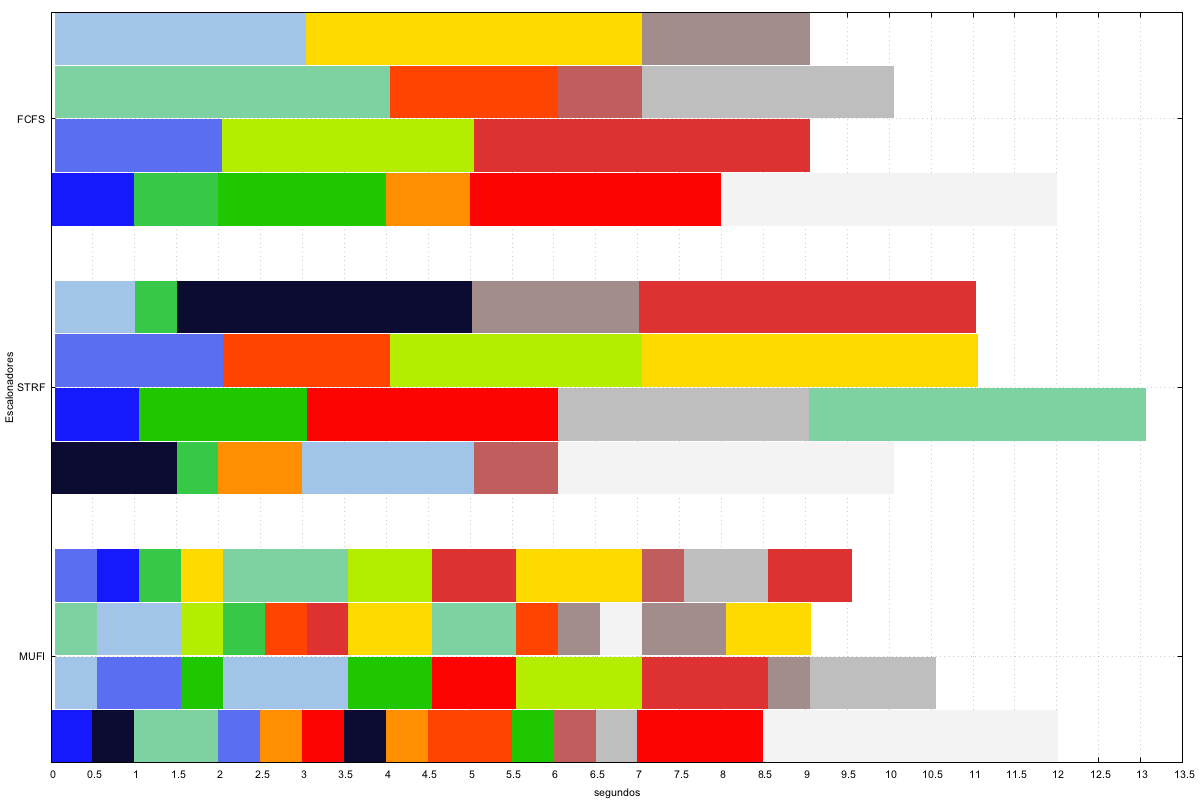
\includegraphics[width=\textwidth]{graphs/comparacao}
\end{frame}

\end{document}